\section{W11 - Planning \& Control Activities}
\subsection{Planning and Control}
\subsubsection{Planning or Control?}
\subsubsection{Definitions}
\subsubsection{Example: Air France Flight Plan: What Do You Have to Plan?}
\subsubsection{Example: SWISS: European Airbus Fleet Flight Plan for one Day }
\subsubsection{Significance of Planning and Control Time horizon Hours/days Days/weeks/months Months/years}
\subsubsection{Dependent and Independent Demand }
\subsubsection{The Order Penetration Point (OPP)}
\subsubsection{Goals to Optimize with the OPP}
\subsection{The 4 Main Activities of P\&C}
\subsubsection{The Activities of Planning and Control}
\subsubsection{Scheduling Using a Gantt Diagram}
\subsubsection{Factors Affecting Operating Time}
\subsubsection{Finite and Infinite Loading of Work Centers}
\index{Loading!Finite}
\index{Loading!Infinite}
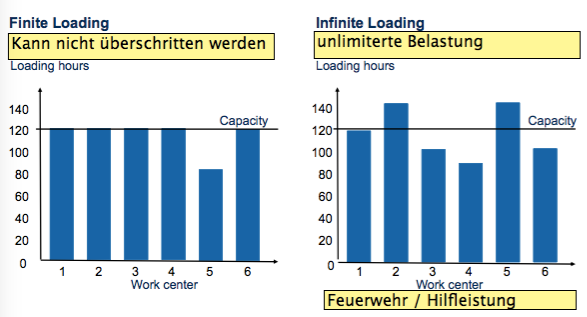
\includegraphics[width=1\textwidth]{W11/finitevsinfinite}
\subsubsection{Local Decision Rules\index{Local Decision Rules}, e.g., Sequencing}
4 jobs for 1 work center may be planned according to the following possibilities:
$4 \cdot 3 \cdot 2 \cdot 1 = 24 possibilities$

n jobs for 1 work center yields $n!$ possibilites of sequencing\index{sequencing}\\
n jobs for m work centres yields $n^m$ possibilities of sequencing.
\subsubsection{Sequencing: Minimizing Throughput Time}
\subsubsection{Gantt Diagram of Your Orders}
\subsubsection{Planning Boards: Visible Communication Tool for Use Between Planning and Production and within Production}
\subsection{Enterprise Resource Planning}
\subsubsection{ERP = Enterprise Resource Planning}
\subsubsection{The Development of ERP}
\subsubsection{Material Requirements Planning (MRP)}
\subsubsection{Total Future Demand Is Made up of Known and Forecast Demand}
\subsubsection{Example: Treasure Hunt Game Product Structure}
\subsubsection{‘Treasure Hunt Game’: Indented Bill of Material}
\subsubsection{ERP Structure for a Sandwich Company}
